%%%%%%
%
% $Autor: Wings $
% $Datum: 2020-01-18 11:15:45Z $
% $Pfad: WuSt/Skript/Produktspezifikation/powerpoint/ImageProcessing.tex $
% $Version: 4620 $
%
%%%%%%

% 
%todo  \url{http://www.industry-analytics.de/ki-wann-sind-maschinen-intelligent/}

%todo         \href{https://dida.do/de/blog/was-ist-ki}{Was ist KI}




\chapter{Künstliche Intelligenz - Wann sind Maschinen intelligent?}

Die Beantwortung der Frage ist nicht einfach. Zunächst muss der Begriff Intelligenz definiert werden. Ihre Definition ist nicht eindeutig.  Beispielsweise ist nicht definiert, ab wann ein Mensch als intelligent gilt. Das bringt die Frage auf, was zur Intelligenz gehört. In der Psychologie wird unter Intelligenz unter anderem die Fähigkeit gezählt, sich an unbekannte Umgebungen und Situationen anzupassen, aber auch neue Probleme zu lösen.\cite{Funke:1998}


\section{Was ist Künstliche Intelligenz?}

Demzufolge ist der Begriff der Künstlichen Intelligenz ebenfalls nicht eindeutig definiert. Historisch wurde der Begriff von John McCarthy eingeführt  \cite{McCarthy:2006}:

\bigskip

\textsl{\glqq Ziel der KI ist es, Maschinen zu entwickeln, die sich verhalten, als verfügten sie über Intelligenz.\grqq{}} - John McCarthy, 1955
	
\bigskip

Gemäß dieser Definition sind einfache Maschinen und Sensoren intelligent. Dabei agieren sie einem Programm folgend. Das heißt, alle Reaktionen des Systems sind vorher ermittelt und festgelegt worden. Falls einzelne Eigenschaften des Menschen betrachtet werden, so können gemäß Definition sehr viele Maschinen als intelligent betrachtet werden; insbesondere da Maschinen Tätigkeiten, die von Menschen ganz oder teilweise durchgeführt werden, übernommen haben. Ein einfaches Beispiel sind Rechenprogramme. Sie sind in diesem Bereich um ein Vielfaches leistungsfähiger als Menschen. Daher findet man auch die folgende Definition \cite{Rich:1983}:


\bigskip

\textsl{\glqq AI is the study of how to make computers do things which, at the moment, people do better.\grqq{}} - Elaine Rich, 1983 
	
\bigskip

Dieser Ansatz ist insofern geschickt, da er die Definition der Intelligenz umgeht. Andererseits weist er darauf hin, dass es sich um eine Momentaufnahme handelt. Dies berücksichtigt, dass der Mensch sehr anpassungsfähig ist. Diese Anpassungsfähigkeit zeichnet ihn insbesondere aus. Der Mensch ist in der Lage, neue äußere Einflüsse zu erfassen und sich darauf anzupassen. Er kann eigenständig lernen.

\bigskip

In der Dekade von 2010 bis 202 wurden sehr viele beeindruckende Ergebisse im Bereich der Künstlichen Intelligenz erreicht. Der Computer  Watson besiegt 2011 den menschlichen Champion in der sehr beliebten Rateshow \glqq Jeopardy\grqq{} \cite{Ferrucci:2012}. Profispieler des Brettspiels Go wurden in den Jahren 2015 und 2016 erstmalig von  System AlphaGo geschlagen \Cite{Wang:2016}. Selbst das Bluffen beim Poker hat eine Künstliche Intelligenz mit dem Namen Libratus 2017 erfolgreich angewendet \cite{Brown:2018}. 2018 zeigt ein Computerprogramm des chinesischen Konzerns Alibaba eine besseres Leseverständnis als Menschen. Die Software GPT-3 schreibt 2020  Sachtext und Gedichte, die wie von Menschenhand erstellt sind. Auch in der Kunstwelt sind Künstliche Intelligenzen tätig geworden; so wurden neue Lieder der Beatles komponiert und Bilder im Stile von berühmten Maler erstellt. Diese Erfolge verleiten zu dem Schluss, dass Computersoftware der menschlichen Intelligenz überlegen ist. Um den Unterschied zu verdeutlichen, werden die Begriffe schwache und starke Intelligenz eingeführt. Starke Künstliche Intelligenz ist für allumfassend entwickelte Software, die sich auch auf andere beziehungsweise neue Anforderungen anpassen kann. Dagegen bedeutet schwache Künstliche Intelligenz, dass ein Algorithmus zum Lösung einer speziellen Aufgabe entwickelt wurde. Sie können komplexe und anspruchsvolle Aufgabe aus sehr unterschiedlichen Bereichen so gut  wie Menschen  oder besser lösen. Die obige Aufzählung zeigt, dass schwache Künstliche Intelligenz atemberaubende Ergebnisse liefern. Aber starke Künstliche Intelligenz gibt es genauso wenig wie eine Zeitmaschine.
%Zeit.de/ 2021/13
In der Grafik~\ref{figKIMLDL} sind die Beziehungen zwischen starker, schwacher Künstlicher Intelligenz, Maschinelles Lernen und Deep Learning dargestellt; demnach ist Deep Learning ein Teilgebiet des Maschinellen Lernens und dies wiederum ein Teilgebiet der Künstlichen Intelligenz.

\begin{figure}
  \begin{center}
    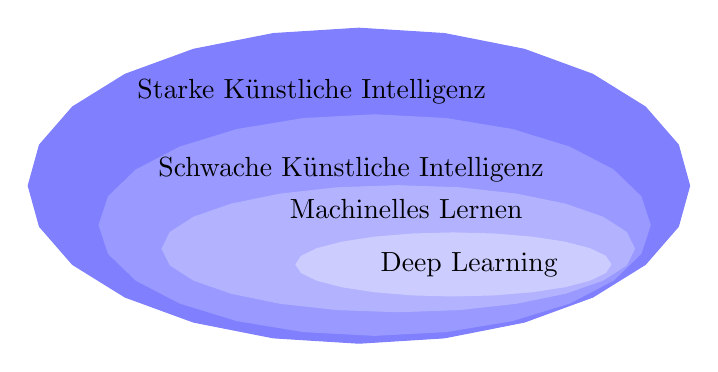
\begin{tikzpicture}
      \draw [blue!50,fill=blue!50,domain=0:360] plot ({-1.2+4.2*cos(\x)}, {0.6+2.0*sin(\x)});
      \draw [blue!40,fill=blue!40,domain=0:360] plot ({-1+3.5*cos(\x)}, {0.1+1.4*sin(\x)});
      \draw [blue!30,fill=blue!30,domain=0:360] plot ({-0.7+3*cos(\x)}, {-0.2+0.8*sin(\x)});
      \draw [blue!20,fill=blue!20,domain=0:360] plot ({2*cos(\x)}, {-0.4+0.4*sin(\x)});
      
      \node (DP) at (0.2,-0.4) {Deep Learning};
      \node (ML) at (-0.6,0.3) {Machinelles Lernen};
      \node (AI) at (-1.3,0.8) {Schwache Künstliche Intelligenz};
      \node (AI) at (-1.8,1.8) {Starke Künstliche Intelligenz};
    \end{tikzpicture}

    \caption{Beziehung von Künstlicher Intelligenz, Maschinelles Lernen und Deep Learning}\label{figKIMLDL}
    \end{center}
\end{figure}


\section{Maschinelles Lernen}

Maschinelles Lernen stellt die Fähigkeit einer Maschine dar, Wissen aus vorliegenden Daten zu extrahieren und Muster zu erkennen. Bei Bedarf kann dieses Muster dann auf darauffolgende Datensätze angewandt werden. Die Art und Weise, wie der Lernvorgang erfolgt, kann dabei in drei Kategorien aufgeteilt werden:

\begin{description}
  \item[Überwachtes] Lernen (Supervised Learning) nutzt für den Lernprozess Trainings- und Testdaten. Die Trainingsdaten beinhalten sowohl Eingangsdaten, zum Beispiel Objektkennzahlen, als auch das gewünschte Ergebnis, zum Beispiel Klassifikation der Objekte. Der Algorithmus soll dann anhand der Trainingsdaten eine Funktion finden, welche die Eingangsdaten auf das Ergebnis abbildet. Hierbei wird die Funktion während des Lernprozesses selbständig von dem Algorithmus angepasst. Wurde eine bestimmte Erfolgsquote für die Trainingsdaten erreicht, wird der Lernprozess mit Hilfe der Testdaten verifiziert. Ein Beispiel hierfür wäre ein Clusteringverfahren, bei dem die Cluster bereits vor Beginn des Lernprozesses bekannt sind. 

  \item [Unbewachtes Lernen] (Unsupervised Learning) nutzt für den Lernprozess lediglich Eingangsdaten, bei denen das Ergebnis noch nicht feststeht. Anhand von den Merkmalen der Eingangsdaten sollen in diesem Muster erkannt werden. Ein Anwendungsgebiet des unbewachten Lernens stellt das Clustering von Daten dar, bei denen die einzelnen Cluster vor dem Lernprozess noch nicht definiert sind. 

  \item [Verstärktes] Lernen (Reinforcement Learning) basiert auf dem Belohnungsprinzip für erfolgte Aktionen. Hierbei wird in einem Ausgangszustand ohne Informationen über das Umfeld oder über dies Auswirkungen von Aktionen begonnen. Eine Aktion führt dann zu einem neuen Zustand und liefert eine Belohnung, die positiv oder negativ ist.  Dies wird solange durchgeführt, bis eine Endbedingung eingetreten ist. Anschließend kann der Lernprozess wiederholt werden, um die Belohnung zu maximieren. 
\end{description}

\section{Deep Learning}
 
Deep Learning stellt einen Teilbereich des Maschinellen Lernens dar und verwendet ein \ac{nn} für den Lernprozess. Diese repräsentieren ein Modell des menschlichen Gehirns und der neuronalen Prozesse. Dabei besteht das \ac{knn} aus Knotenpunkte, welche Neuronen repräsentieren. Hierbei wird zwischen drei Kategorien von Neuronen unterschieden. 

%\GRAPHICSC{1.0}{1.0}{kdd/Knn}


\begin{figure}
  \begin{center}
    
    \def\layersep{2.5cm}
    
    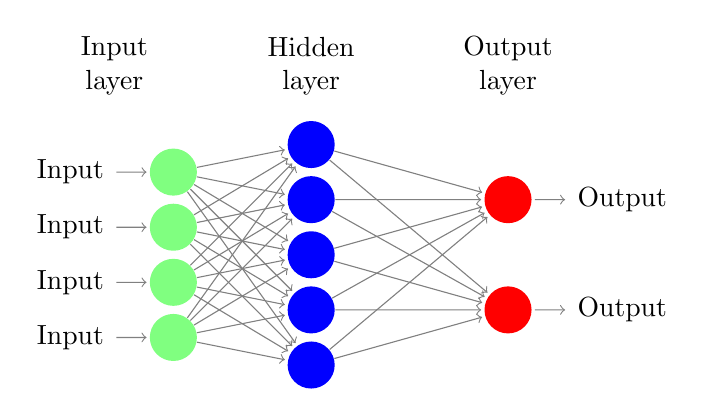
\begin{tikzpicture}[shorten >=1pt,->,draw=black!50, node distance=\layersep,scale=0.7]
      \tikzstyle{every pin edge}=[<-,shorten <=1pt]
      \tikzstyle{neuron}=[circle,fill=black!25,minimum size=17pt,inner sep=0pt]
      \tikzstyle{input neuron}=[neuron, fill=green!50];
      \tikzstyle{output neuron}=[neuron, fill=red];
      \tikzstyle{hidden neuron}=[neuron, fill=blue];
      \tikzstyle{annot} = [text width=4em, text centered]
        
      % Draw the input layer nodes
      \foreach \name / \y in {1,...,4}
        % This is the same as writing \foreach \name / \y in {1/1,2/2,3/3,4/4}
        \node[input neuron, pin=left:Input] (I-\name) at (0,-\y) {};
        
        % Draw the hidden layer nodes
      \foreach \name / \y in {1,...,5}
        \path[yshift=0.5cm]
        node[hidden neuron] (H-\name) at (\layersep,-\y cm) {};
        
        % Draw the output layer node
        \node[output neuron,pin={[pin edge={->}]right:Output}, right of=H-2] (O1) {};
        \node[output neuron,pin={[pin edge={->}]right:Output}, right of=H-4] (O2) {};
        
        % Connect every node in the input layer with every node in the
        % hidden layer.
        \foreach \source in {1,...,4}
          \foreach \dest in {1,...,5}
            \path (I-\source) edge (H-\dest);
        
        % Connect every node in the hidden layer with the output layer
        \foreach \source in {1,...,5}
          \path (H-\source) edge (O1);
        \foreach \source in {1,...,5}
          \path (H-\source) edge (O2);
        
        % Annotate the layers
        \node[annot,above of=H-1, node distance=1cm] (hl) {Hidden layer};
        \node[annot,left of=hl] {Input layer};
        \node[annot,right of=hl] {Output layer};
    \end{tikzpicture}
  \end{center}
  \caption{Beispiel eines \ac{knn}}\label{fig:knn}
\end{figure}


\begin{description}
  \item[Input-Neuronen]  sind die Neuronen, welche Signale von der Außenwelt empfangen. Hier gibt es für jede Art von Input (Merkmal/Feature) ein Neuron.
  \item[Hidden-Neuronen] sind Neuronen, welche den eigentlichen Lernprozess repräsentieren.
  \item [Output-Neuronen]  sind die Neuronen, welche Signale an die Außenwelt abgeben. Hierbei gibt es für jede Art von Output (Merkmal/Feature) ein Neuron.
\end{description}

\bigskip

Alle Neuronen einer Kategorie werden zu einer Schicht, Layer genannt, zusammengefasst. Somit gibt es in jedem neuronalen Netzwerk einen Input-Layer, siehe Abbildung\ref{fig:knn} grüne Neuronen, einen Hidden Layer, in der Abbildung~\ref{fig:knn} die blauen Neuronen, und einen Output Layer mit den roten Neuronen in der Abbildung~\ref{fig:knn}. Enthält ein \ac{knn} mehr als einen Hidden Layer wird es als Deep Neural Network bezeichnet. Die Verbindungen zwischen den  Neuronen der einzelnen Layer werden als Synapsen bezeichnet. Diese enthalten eine Gewichtung, welche mit dem Signal des Startneurons multipliziert werden. Somit werden die einzelnen Signale gewichtet. Die Gewichte werden wiederum während des Lernprozesses, basierend auf Funktionen, angepasst.


\section{Anwendung}

Aufgrund der Anpassungsfähigkeiten von Künstlichen Intelligenzen sind diese vielfältig einsetzbar. McKinsey hat der Studie \glqq Smartening up with Artificial Intelligence (AI)\grqq{} acht Anwendungsszenarien beschrieben, in welchem Künstliche Intelligenz besonders Potenziale aufweist \cite{McKinsey:2017}.

\begin{itemize}
  \item Autonome Fahrzeuge
  \item Predictive Maintenance durch bessere Vorhersagen 
  \item Gemeinschaftlich agierende Robotik mit Wahrnehmung der Umgebung (Maschine-Maschine-Interaktion \& Mensch-Maschine-Interaktion)
  \item Qualitätssteigerung durch selbstständiges Anpassen von Maschinen an zu verarbeitende Produkte
  \item Automatisierte Qualitätsprüfung
  \item Supply-Chain-Management durch genauere Vorhersagen
  \item Forschung und Entwicklung
  \item Automatisierte Unterstützung von Prozessen
\end{itemize}


%todo Gedanke industrie 4.0 / Edge-Computer ist gut, sonst raus


%Wenn es einen Bereich gibt, der prägend für das 21. Jahrhundert ist, dann mit Sicherheit
%die Künstliche Intelligenz, die uns heutzutage in vielen Dingen des Alltags begegnet.
%Im privaten Rahmen haben sich beispielsweise persönliche Sprachassistenten, wie zum Beispiel
%Alexa von Amazon, in viele Haushalte integriert. Diese beantworten über Sprachbefehle
%alle Fragen, schalten auf Befehl das Licht an oder spielen die Lieblingsmusik. Im 
%industriellen Umfeld forschen große Automobilbranchen daran, dass autonome Fahren weiter
%voranzubringen und mit Hilfe der künstlichen Intelligenz den Straßenverkehr sicherer zu
%gestalten.
%
%Das Grundprinzip der künstlichen Intelligenz existiert schon seit Ende der 1950er, doch
%hat es erst mit dem technischen Fortschritt in der Computerindustrie und der zunehmenden 
%Vernetzung der Welt sein Potential weiter entfalten können. Die Bundesregierung
%in Deutschland hat großes Interesse daran, die Entwicklung der künstlichen Intelligenz
%schnell voranzutreiben, um weltweit die Wettbewerbsfähig zu sicher und fördert Projekte
%in diesem Bereich mit Milliardenpaketen. \cite{Hubel:1959,Werle:2020} 
%
%Besonders interessant ist diese Technologie für Unternehmen, die sich nach den Grundsätzen
%der \glqq Industrie 4.0\grqq{} weiterentwickeln wollen. Grundlegendes Ziel dabei ist, 
%das Eingreifen des Menschen in den Produktionsprozess zu minimieren und die digitale 
%Kommunikation von Anlagen untereinander zu maximieren. Der Produktionsprozess soll dadurch 
%transparenter gestaltet und optimiert werden. Besonders gut dafür geeignet sind 
%Edge-Computing-Systeme, welche Daten dezentral und in Echtzeit verarbeiten und auswerten 
%können. Die daraus resultierenden Ergebnisse können anschließend an einen zentralen Server 
%weitergeleitet werden. \cite{Martins:2019}
%
%Als Werkzeug zur Steigerung von Effizienz und Effektivität industrieller Prozesse, auch 
%durch einen höheren Autonomiegrad, spielt die künstliche Intelligenz eine wichtige Rolle.
%Im Feld, dem sogenannten Edge-Bereich, können Systeme für künstliche Intelligent
%von jedem durch Systeme wie den Jetson Nano entwickelt und erprobt werden.
%\cite{JetsonProjects:2020}
%
%
%
%
%%\glqq Die Künstliche Intelligenz, kurz KI, einfach erklärt, ist der Versuch, menschliches Lernen und Denken auf den Computer zu übertragen und ihm damit Intelligenz zu verleihen. Statt für jeden Zweck programmiert zu werden, kann eine KI eigenständig Antworten finden und selbstständig Probleme lösen.\grqq{} \cite{KI:2020}
%%
%%\bigskip
%
%
